\section{Введение в \cmsis}\label{cmsisintro}

\cp{двойной лось
\url{http://www.doulos.com/knowhow/arm/CMSIS/CMSIS\_Doulos\_Tutorial.pdf}}

Cortex Microcontroller Software Interface Standard (CMSIS)\footnote{стандарт
программного интерфейса микроконтроллеров Cortex}\ обеспечивает разработчикам и
производителям МК создание повторно используемых программных компонентов для
систем на основе микроконтроллеров \cm{}.

Процессор \arm\ \cm{3}\ первое ядро от компании \arm\ специально разработанное
для рынка микроконтроллеров. Это ядро включает множество типовых блоков (NVIC,
таймеры, отладочный интрефейс) необходимых на этом рынке. Это позволяет
разработчикам с минимальными усилиями портировать и повторно использовать уже
написанное ПО\footnote{например ядро ОС реального времени}\ для МК семейства
\cm{3}\ любых производителей.

Благодаря идентичности большого колиства аппаратных компонентов, также
идентичным оказывается и Hardware Abstraction Layer (HAL)\footnote{программный
слой аппаратной абстракции}.
Тем не менее, реальность показывает что отсутствие общего стандарта приводит к
множеству несовместимых версий библотек HAL и драйверов для различных МК, что не
соответствует идее полной переносимости ПО в серии \cm{3}.

Последние исследования разработок для рынка встраиваемого ПО показывают, что
сложность программного обеспечения и его стоимость постоянно увеличиваются.
Повторное использование кода и наличие общего стандарта управляющего способами
написания и отладки ПО необходимы для минимизации стоимости разработки и
сопровождения.

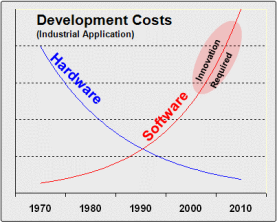
\includegraphics[height=30ex]{fig/cmsisdevcosts.png}
стоимости разработки

\bigskip
Анализируя ситуацию с взрывным ростом количества моделей МК \cm{3}\ на рынке,
компания \arm\ обнаружила что полная идентичность аппаратной части недостаточна
для обеспечения совместимости, и необходимо создание стандарта доступа к
аппаратным компонентам.

Результатом этих исследований является \cmsis: фреймворк, расширямый
поставщиками МК, с сохранением полезных свойств общего API (Application Programming
Interface)\footnote{прикладной программный интерфейс} для ядреных компонентов и
соглашениями о том, как должны быть реализованы части зависимые от железа, чтобы
разработчики чувствовали себя как дома при повторном использовании ил разработки
нового кода для семейства \cm{}.

\subsection{Структура \cmsis}

\cmsis\ может быть поделен на три основных слоя:

\begin{enumerate}
\item Core Peripheral Access Layer (CPAL)

Самый нижний уровень определяет адреса, и методы доступа к общим компонентам и
функциям, существующим в каждой \cm{}-системе. Этим уровнем
описывается доступ к регистрам ядра, NVIC\footnote{Nested Vector Interrupt
Controller, контроллер вложенных прерываний}, подсистеме отладки.
Инструментальный доступ к спецрегистрам (\file{CONTROL},\file{xPSR})
предоставляется в форме inline-функций или интринсик компилятора. Этот уровень
обеспечивается лицензиатом архитектуры\ --- компанией \arm.

\item Middleware Access Layer (MWAL)

Этот слой также специфицируется \arm, но адаптируется производителем кристаллов
для их конкретных изделий. Слой MWAL определяет общий API для доступа к
периферии. Этот слой все еще находится на стадии доработки, и на текущий момент
более подробная информация неступна.

\item Device Peripheral Access Layer (DPAL)

Слой содержит адреса аппаратных регистров и другие определения, в том числе
функции доступа к специфичным особенностям чипов.
DPAL сильно похож на CPAL, но предоставляется поставщиком кристаллов.
В CPAL могут быть описаны методы доступа и адаптированная таблица векторов,
содержащая обработчики исключений, специфичные для конкретного МК.

\end{enumerate} 

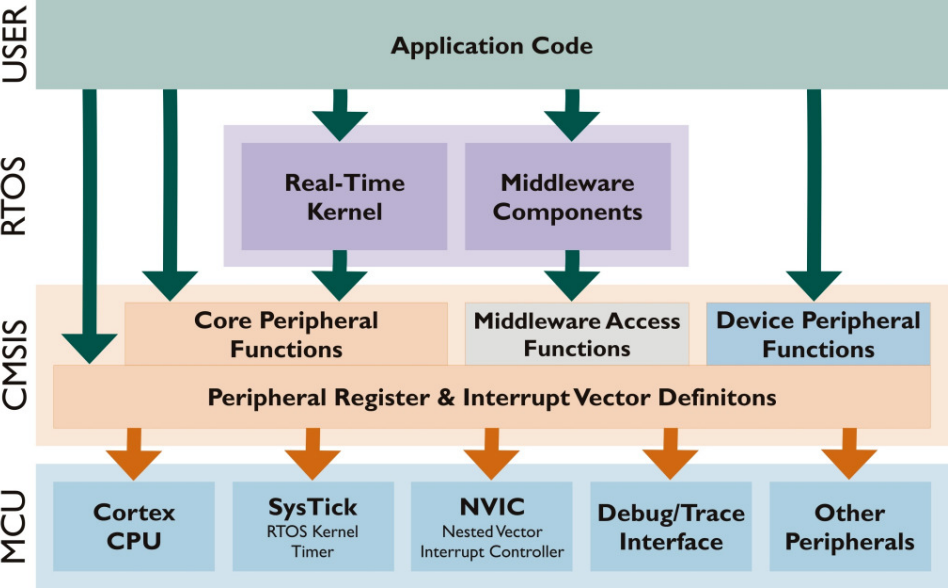
\includegraphics[width=0.9\textwidth]{fig/cmsisstruc.png}

